\documentclass[border=6pt]{standalone}
\usepackage{tikz}
\usetikzlibrary{arrows.meta,positioning,calc,shapes.geometric,fit,backgrounds,patterns,matrix,decorations.pathreplacing}
\begin{document}
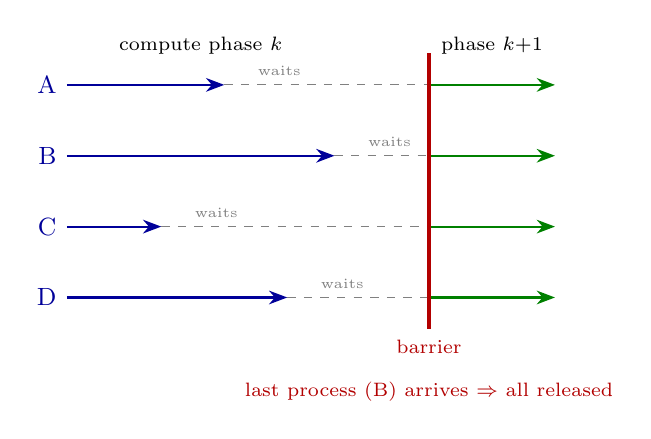
\begin{tikzpicture}[>=Stealth,font=\small]
\foreach \p/\t/\n in {0/2.0/A,1/3.4/B,2/1.2/C,3/2.8/D}
{ \draw[->,thick,blue!60!black] (0,-\p*0.9) node[left]{\n} -- (\t,-\p*0.9);
  \draw[dashed,gray] (\t,-\p*0.9) -- (4.6,-\p*0.9);
  \draw[->,thick,green!50!black] (4.6,-\p*0.9) -- (6.2,-\p*0.9);
  \node[font=\tiny,gray] at (\t+0.7,-\p*0.9+0.18) {waits}; }
\draw[very thick,red!70!black] (4.6,0.4) -- (4.6,-3.1) node[below,font=\scriptsize]{barrier};
\node[font=\scriptsize] at (1.7,0.5) {compute phase $k$};\node[font=\scriptsize] at (5.4,0.5) {phase $k{+}1$};
\node[font=\scriptsize,red!70!black,align=center] at (4.6,-3.9) {last process (B) arrives $\Rightarrow$ all released};
\end{tikzpicture}
\end{document}
